\documentclass[oneside, astronomy, noacknowlegments]{BYUPhys}
% Your name
  \Author{Scott Leland Crossen}

% Enter the date your thesis is approved
  \Year{[Year]}
  \Month{[Approval Month]}

% If you have a long title, split it between multiple lines using the \\ command
  \Title{Optically Detected Magnetic Resonance\index{Optically Detected Magnetic Resonance (ODMR)}; Computational Predictions\\and Experimental Results
  }

% Your research advisor
\AdvisorTitle{Advisor}
  \Advisor{Dr. John S. Colton}

% For honors theses, enter the name of the honors Representative
  \HonorsRepresentative{Kristine Hansen}

% The text of your abstract
  \Abstract{ \textit{Electron Spin Resonance}\index{Electron Spin Resonance (ESR)}\index{Electron Paramagnetic Resonance (EPR)} (ESR\index{Electron Spin Resonance (ESR)}\index{Electron Paramagnetic Resonance (EPR)}) is an important tool in understanding the quantum-mechanical properties of condensed matter. It's applications range from studying lattice-defect\index{lattice-defects} in solids to studying spin coherence in qubit candidate materials used for quantum computing\index{quantum computing}. When coupled with a photoluminesce measuring component, a double-resonance-technique allows for optical readout of ESR\index{Electron Spin Resonance (ESR)}\index{Electron Paramagnetic Resonance (EPR)} information. This unique form of ESR\index{Electron Spin Resonance (ESR)}\index{Electron Paramagnetic Resonance (EPR)} is called \textit{Optically Detected Magnetic Resonance\index{Optically Detected Magnetic Resonance (ODMR)}} (ODMR\index{Optically Detected Magnetic Resonance (ODMR)}). In this thesis we compare experimental ODMR\index{Optically Detected Magnetic Resonance (ODMR)} data with ESR\index{Electron Spin Resonance (ESR)}\index{Electron Paramagnetic Resonance (EPR)} predictions generated from computational modelling systems. To investigate the differences between these two methods we will study two spin-systems in particular: irradiated 4H silicon carbide\index{silicon carbide (4H SiC)} and thin-film cadmium telluride\index{cadmium telluride (CdTe)}. These two specimens will serve as the primary means to connect experimentally and theoretically the two very different forms of computational and practical ESR\index{Electron Spin Resonance (ESR)}\index{Electron Paramagnetic Resonance (EPR)} spectroscopy commonly used today. Methods and theory for both methods will be described and resulting spectrums will be overlaid for comparison. Though there will always be some differences, results show that computational ESR\index{Electron Spin Resonance (ESR)}\index{Electron Paramagnetic Resonance (EPR)} predictions match experimental results to the same extent that the underlying Hamiltonian for that particular system is understood. }

 \Keywords{[A comma-separated list of descriptive words for search purposes]}

% Acknowledge those who helped and supported you
  \Acknowledgments{
    [Acknowledgements should be simple, in good taste, and fit on one page]
  }

%% The members of your committee (masters only need A and B, PhD need all 4)
%  \MemberA{Committee Member A}
%  \MemberB{Committee Member B}
%  \MemberC{Committee Member C}
%  \MemberD{Committee Member D}
%

\begin{document}

 % Start page counting in roman numerals
 \frontmatter

 % This command makes the formal preliminary pages.
 % You can comment it out during the drafting process if you want to save paper.
 \makepreliminarypages

 % Make the table of contents.
 \tableofcontents

 % Start regular page counting at page 1
 \mainmatter

 % Include a list of figures
 \listoffigures 








\chapter{Introduction}

\section{Qualitative Description of ESR\index{Electron Spin Resonance (ESR)}\index{Electron Paramagnetic Resonance (EPR)} and ODMR\index{Optically Detected Magnetic Resonance (ODMR)}}
\label{sec:qualitative}

\textit{Optically Detected Magnetic Resonance\index{Optically Detected Magnetic Resonance (ODMR)}} (ODMR\index{Optically Detected Magnetic Resonance (ODMR)}) is a particular form of \textit{Electron Paramagnetic Resonance\index{Electron Spin Resonance (ESR)}\index{Electron Paramagnetic Resonance (EPR)}} (EPR\index{Electron Spin Resonance (ESR)}\index{Electron Paramagnetic Resonance (EPR)}) which is more commonly known as \textit{Electron Spin Resonance\index{Electron Spin Resonance (ESR)}\index{Electron Paramagnetic Resonance (EPR)}} (ESR\index{Electron Spin Resonance (ESR)}\index{Electron Paramagnetic Resonance (EPR)}). The latter two of these terms (EPR and ESR\index{Electron Spin Resonance (ESR)}\index{Electron Paramagnetic Resonance (EPR)}) are synonymous; The former (ODMR\index{Optically Detected Magnetic Resonance (ODMR)}) is a particular subset of ESR\index{Electron Spin Resonance (ESR)}\index{Electron Paramagnetic Resonance (EPR)} that utilizes a luminescence measuring technique as a means to collect ESR\index{Electron Spin Resonance (ESR)}\index{Electron Paramagnetic Resonance (EPR)} information. In literature, it is common to see both of these terms followed by the designation ``spectroscopy" which signifies that they are tools to study properties of matter via electromagnetic radiation. Though the extent of their application has grown over the years, ESR\index{Electron Spin Resonance (ESR)}\index{Electron Paramagnetic Resonance (EPR)} and ODMR\index{Optically Detected Magnetic Resonance (ODMR)} are most commonly used to study the spin-properties of electrons and electron-holes trapped in metal lattices. They can be used to study free radicals in organic materials and are also important in studying the local environment of lattice defects\index{lattice-defects} through a technique using angular-dependent ODMR\index{Optically Detected Magnetic Resonance (ODMR)}. One particular use of ODMR\index{Optically Detected Magnetic Resonance (ODMR)} is the study of electron-spin coherence via a technique known as \textit{Electron Spin Echo}. This can be useful when studying what properties and conditions lead to superior state coherence for qubit candidate materials in quantum computing\index{quantum computing}.

The intellectual foundation of Electron Spin Resonance\index{Electron Spin Resonance (ESR)}\index{Electron Paramagnetic Resonance (EPR)} is rooted in Quantum Mechanics. Bound electrons in matter have discrete and quantized energy levels that govern what frequencies of light are emitted when transitions between energy levels are made. For electron systems, which are fermions and thus subject to the Pauli exclusion principle, the energy levels are 2nd order degenerate when bound in matter. In Quantum Mechanics we choose to describe this degeneracy in terms of spins: we say an electron is either ``spin-up" or ``spin-down". Each energy level can have at most two electrons of opposite spins inhabiting it (and thus the degeneracy). The spin terminology is arbitrary however, and is really just an attempt at comparing electrons to particles. In truth, electron spin is a term for a property that is emergent from solving the wave equation. However, it nonetheless describes the principle of conservation of momentum that would be found in classical system such as a top and so the term makes sense and has persisted in usage today. In this case, the electron's spin is a description of the magnetic moment for when the particle is in the presence of a magnetic field. In the case of electrons bound in matter within a magnetic field, the energy levels of the molecule will split according to the ``Zeeman Effect" and the spin-states of the electrons can be observed - most commonly through a photoluminescence or other fluorescence measuring technique.

The Zeeman effect itself is crucial in understanding the principles of ESR\index{Electron Spin Resonance (ESR)}\index{Electron Paramagnetic Resonance (EPR)}. In the presence of a magnetic field, populations of free electrons will form a spin-1/2 system between a higher-energy ``spin-up" state and a lower-energy ``spin-down" state. In matter, different parities of spin-states can be formed between the interactions of different energy levels with different transition selection rules. A spin-1/2 system in the presence of a magnetic field is shown in \ref{fig:Zeeman}. As seen here, the energy levels of the two differing spins diverge linearly for an increasing magnetic field. The difference in energy between these two levels is typically in the microwave frequency domain. For a given magnetic-field strength there will be a set of characteristic microwave frequencies that the electrons are most prone to emitting when transitioning between these quantized states. In a spin-1/2 system there will only be one frequency for a given magnetic field corresponding to the difference between the two Zeeman lines at the given field strength. Likewise, for a given microwave target signal, there will be a variety of magnetic field strengths which are most adept at transitioning bound electrons between states. This unique pairing between both the microwave frequency and magnetic field strength is the resonant condition upon which ESR\index{Electron Spin Resonance (ESR)}\index{Electron Paramagnetic Resonance (EPR)} is based off of and also the means it uses to discover information about materials.

\begin{figure}
    \centerline{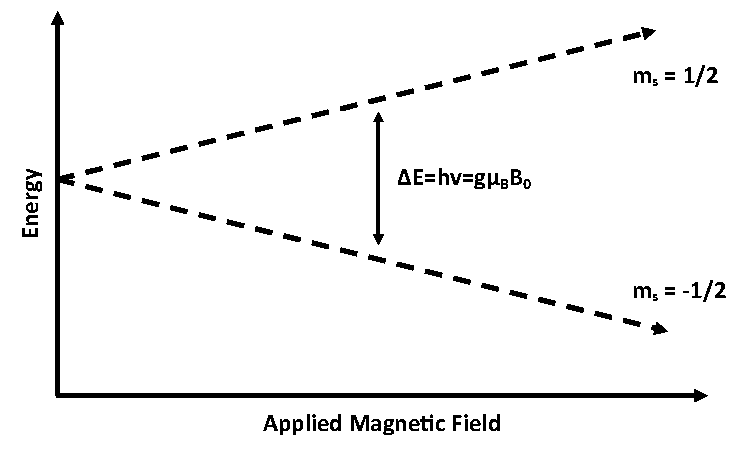
\includegraphics{zeeman_fig}}
    \caption[Zeeman effect and resonant conditions in matter]{\label{fig:Zeeman}
     Zeeman effect for a two level system showing spin ( $\pm 1/2$ ) energy levels as a function of applied magnetic field. For arbitrary field strength the energy difference is shown as a function of $\mu$, $g$, and the field strength $B$.}
\end{figure}

\section{The Defect\index{lattice-defects} Nature of Materials}

[Rough - More] In solid-state physics, materials form crystal lattices for molecular tessellation. These structures are not perfect, however, and often have intrinsic interstitial defects\index{lattice-defects}. These defects\index{lattice-defects} come in the form of either additional or missing atoms. [continued]

[Rough - More] Crystal lattice defects\index{lattice-defects} are important as they contribute to the overall spin system of the material via either electrons or electron-holes.

[Rough - More] Optically Detected Magnetic Resonance\index{Optically Detected Magnetic Resonance (ODMR)} (ODMR\index{Optically Detected Magnetic Resonance (ODMR)}) can be used in conjunction with a varied applied angle (between the magnetic field and c-plane) to study the local nature of each type of defect\index{lattice-defects} in the material.

[Rough - More] ODMR\index{Optically Detected Magnetic Resonance (ODMR)} can give the information necessary in understanding how the lattice is formed.

[Rough - More] Defects\index{lattice-defects} can be introduced via high-fluence irradiation of particles.

\section{Electron Spin, Quantum Computing\index{quantum computing}, and Qubits}

Classical Computation is almost always based upon a binary system. In these architectures, the computer's register, memory, and general logical states are either in a logical `true' or a logical `false' state. A `true' state corresponds to a high voltage and a `false' state corresponds to a grounded voltage. A computer's bits can be in either of these two states - 1 or 0 - but not both.

A spin-1/2 system also describes a binary system between a higher-energy basis state and a lower-energy basis state. In this comparison, the spin-1/2 system will be measured (and the wave function collapsed) to be in either of these two states - but not both. The important difference between the the spin-1/2 system and the classical computer bit model is that the spin system can have states that exist as linear combinations of the two basis up/down states. In accordance with Quantum Mechanics, this means that the spin-1/2 system can exist as a superposition between both the spin-up and spin-down states and has a certain probability of being measured in each. It is important to note that this superposition does not mean that the state exists as some value in between an excited state and a lower state. Rather, it exists with some value in both states simultaneously.

Because of this unique property of spin systems, they can be used as a basis for forming what is called a ``quantum computer\index{quantum computing}". Though it largely depends on the architecture, Quantum computers\index{quantum computing} can be thought of to manipulate information in a similar fashion to that of a classical computer. Both have logical operators and storage bits and both are algorithmically based. Quantum computers\index{quantum computing}, however, utilize this unique possibility of superposition to make probabilistic calculations for many different states at the same time. This happens through the quantum mechanical operators that initialize and manipulate the states that are stored in ``qubits" - or the quantum computer's\index{quantum computing} version of classical bits that can exist in these superposition types of states. Because of the existing theoretical construction from nondeterministic finite automata to deterministic finite automata, quantum computers\index{quantum computing} are also ``turing complete" in the broad definition of that term. This statement is trivial however, because quantum computers\index{quantum computing} can be operated in the discrete binary limit and so should be able to do anything a classical computer can.

Today, there is large emphasis within the scientific community in building viable, scalable quantum computers\index{quantum computing}. The reason for this is that quantum computers\index{quantum computing} offer reduced computational time limits for certain types of algorithms. Certainly however, these machines are not necessarily more adept at common tasks such as processing videos to be scrubbed by common users, but are rather designed to carry out a few types of intense calculations in logarithmic time that would normally have a polynomial time dependence. The most notable use for quantum computers\index{quantum computing} in our modern society is within the field of computer security and encryption. Quantum computers\index{quantum computing} have the ability to compute prime factors via Shor's algorithm in a much faster time than traditional computers. This ability would essentially render all of the current RSA encryption methods obsolete in addition to anything that relies on public/private key encryption such as bitcoin.

Although more than just spin systems can be used as the all-important qubits for quantum computing\index{quantum computing}, we will focus on this type - specifically spin-1/2 systems formed from electrons - for the basis of our discussion. As mentioned earlier, ESR\index{Electron Spin Resonance (ESR)}\index{Electron Paramagnetic Resonance (EPR)} is the major tool used to study the spin properties of materials. In the case of quantum computation\index{quantum computing}, ESR\index{Electron Spin Resonance (ESR)}\index{Electron Paramagnetic Resonance (EPR)} is used to study possible qubit materials that might eventually be used in such machines. Currently, one of the major difficulties in creating quantum computers\index{quantum computing} is finding materials that can form superposition states that remain coherent (and reliable) over prolonged periods of time. In order to understand what properties of materials lead to superior qubit construction and state coherence, ESR\index{Electron Spin Resonance (ESR)}\index{Electron Paramagnetic Resonance (EPR)} can be used in conjunction with electron spin echo experiments to study the coherence of electrons in a spin-1/2 system. Moreover, ESR\index{Electron Spin Resonance (ESR)}\index{Electron Paramagnetic Resonance (EPR)} can be used alone to study the spin system itself and the local environment of the defects\index{lattice-defects} in materials that form them. Knowledge of this important topic will serve to increase our ability to construct better qubits for use in quantum computers\index{quantum computing}.

\section{Previous Work (Our Research Group and Others)}

\subsection{Preliminary Work and Results}

The work performed in this thesis references in large part the work done by Kyle Miller and Jacob Embley - two students who worked under Dr. John Colton and have since graduated from Brigham Young University. Their work was mostly performed on the topic of Electron Spin Coherence in Proton-Irradiated Silicon Carbide and is documented in their senior theses both of related titles. This thesis, however, will not be on the same topic as the former two but will expand on one aspect used by both of these two students in their work - ODMR\index{Optically Detected Magnetic Resonance (ODMR)}. In addition, both Miller and Embley used a particular species of SiC\index{silicon carbide (4H SiC)} which is one of the two principal materials of investigation in this thesis.

Appendix \ref{chpt:AppendC} includes a publication that Embley, Colton, Miller, myself and a few others produced on the topic of spin coherence in proton irradiated silicon carbide\index{silicon carbide (4H SiC)}. It has been accepted by \textit{Physical Review B} and will appear in publication later in the year 2017. This publication serves as a capstone to the work of both Embley and Miller as included in their senior theses and will serve as the context for which this thesis was produced.

In addition to the work done by Miller and Embley, an additional study was performed on a similar material of the SiC\index{silicon carbide (4H SiC)} specimen which is not included in either the aforementioned theses or publication. This project is included in Appendix \ref{chpt:AppendA}. The major difference with Appendix \ref{chpt:AppendA} and the theses produced by Miller and Embley is the fluence of irradiation used on the SiC\index{silicon carbide (4H SiC)} sample in question. Miller's work was primarily concerned with a $10^{14}$ $cm^{-2}$ proton-irradiated sample of SiC\index{silicon carbide (4H SiC)}. Embley likewise worked with a $10^{13}$ $cm^{-2}$ proton-irradiated sample of SiC\index{silicon carbide (4H SiC)}. In Appendix \ref{chpt:AppendA} I work with a $10^{17}$ $cm^{-2}$ electron-irradiated sample of SiC\index{silicon carbide (4H SiC)} in much the same way as used by Embley. With this additional sample, a more comprehensive analysis and additional results are presented.

\subsection{Experimental Setup}

The experimental setup used for the majority of this thesis was set up and tested by Kyle Miller and Jacob Embley. Miller initially set up all the necessary instrumentation to be used in his experiment which is detailed in his thesis. Later, Embley improved upon most of Miller's design and achieved increased precision and improved results. The experiment used by both Embley and Miller was eventually repurposed and slightly modified for the experiment detailed in this thesis. A full summary and implementation of the experimental setup can be found in \ref{sec:Experiment}. This section includes both the setup used by Miller and Embley as well as the components I modified for the purposes of performing this work.

\subsection{Samples and Collaborative Efforts}

The work done for this thesis was done in collaboration with two groups of people. Firstly, the silicon carbide\index{silicon carbide (4H SiC)} samples used were produced and partially characterized by Dr. Sam Carter of the Naval Research Lab. These samples were irradiated with different fluences of particles in order to introduce different concentrations of defects\index{lattice-defects} into the material. It was Carter's work that ultimately led us to obtain such high quality samples for optical characterization and Electron Spin Resonance\index{Electron Spin Resonance (ESR)}\index{Electron Paramagnetic Resonance (EPR)} studies.

The second collaborative group that we worked with was Dr. Mike Scarpulla of the University of Utah. Scarpulla was responsible for providing the second species of material (CdTe\index{cadmium telluride (CdTe)}) that was characterized for this report. Like the SiC\index{silicon carbide (4H SiC)}, this sample was provided with partial characterization and given to us for optical study. Appendix \ref{chpt:AppendB} gives the full report (at least up to the publication date of this thesis) for the optical studies performed on the CdTe\index{cadmium telluride (CdTe)} sample.

\subsection{Preliminary Results of Experimental ODMR\index{Optically Detected Magnetic Resonance (ODMR)}}

The work done for this thesis is based around two different materials. The first, SiC\index{silicon carbide (4H SiC)}, has had prior work done on it for ODMR\index{Optically Detected Magnetic Resonance (ODMR)} characterization. The second sample, CdTe\index{cadmium telluride (CdTe)}, was not optically characterized for this work prior to our experimentation and was left to us for detailed analysis.

[Rough] Dr. Sam Carter of the Naval Research Lab provided the samples for the silicon carbide\index{silicon carbide (4H SiC)} used. In addition, he also presented a series of plots to describe the spin system present in the material. According to the information he provided, the silicon vacancies in silicon carbide\index{silicon carbide (4H SiC)} form a spin-3/2 system with a metastable doublet state to allow for non-radiative transitions. Another interesting characteristic of this system is that it has a zero-field splitting effect which accounts for a difference of energies without a magnetic field between the spin states +1/2 and +3/2 with -1/2 and -3/2.

In addition to the information provided by Dr. Carter regarding the spin system of SiC\index{silicon carbide (4H SiC)}, he also provided preliminary ODMR\index{Optically Detected Magnetic Resonance (ODMR)} results performed at low field strengths of around 31 mT. The results of his measurements are found in \ref{fig:PrelimODMR} and show the transitions between different spin states which will be more fully developed in \ref{sec:SiCSamples}. Moreover, Carter also provided angular dependent measurements of the resonant relationship between magnetic field strength and microwave frequency. As mentioned in \ref{sec:qualitative}, there exists a unique pairing between the applied magnetic field and the resonant microwave energy transition. For a given magnetic field there will exist different resonant frequencies depending on the spin system in question. In addition, these characteristic frequencies will have associated linewidths that describe what range of frequencies the gaussian distribution is centered around and how wide it is. For the case of a spin-3/2 system as found in 4H-SiC\index{silicon carbide (4H SiC)}, the relationship is best represented by \ref{fig:MFRelationship} which is a plot produced by Dr. Carter for the samples used in this project.

\begin{figure}
    \caption[Magnetic field and microwave frequency relationship]{\label{fig:MFRelationship}
     The relationship between magnetic field strength and microwave Frequency for 4H-SiC\index{silicon carbide (4H SiC)}, a spin-3/2 system. Resonant conditions are shown via bright coloration on the axes of frequency vs field. Notice the linear dependence between both microwave energy and field strength.}
 \end{figure}
 
\begin{figure}
    \centerline{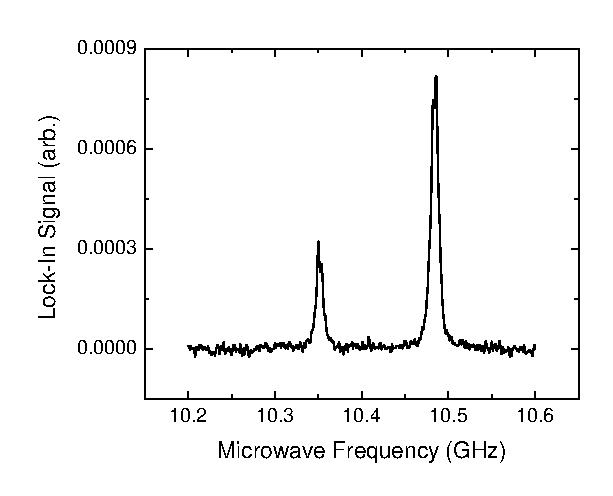
\includegraphics{p14-odmr}}
    \caption[Preliminary ODMR\index{Optically Detected Magnetic Resonance (ODMR)} data]{\label{fig:PrelimODMR}
     The preliminary ODMR\index{Optically Detected Magnetic Resonance (ODMR)} data for Proton Irradiated Silicon Carbide in a constant magnetic field of 2.455 Tesla. The plot shows resonant paramagnetic conditions at 10.35 GHz and 10.47 GHz where the absorption is greatest. }
\end{figure}

\subsection{\textit{EasySpin\index{EasySpin}} Computational Modeling System}

\textit{EasySpin\index{EasySpin}} is a library for \textsc{matlab} designed to computationally model ESR\index{Electron Spin Resonance (ESR)}\index{Electron Paramagnetic Resonance (EPR)} data. The majority of computational work for this thesis was done using this program which was provided free of charge by the vendor's website. Though most of the necessary functions to model ESR\index{Electron Spin Resonance (ESR)}\index{Electron Paramagnetic Resonance (EPR)} data were included in the \textit{EasySpin\index{EasySpin}} library, I still found it necessary to create custom definitions in addition to what was already supplied.

\section{Overview of Thesis}

The purpose of this thesis is to describe in detail the methods and procedures behind experimental and theoretical ESR\index{Electron Spin Resonance (ESR)}\index{Electron Paramagnetic Resonance (EPR)} and to answer the question as to how both experimental and theoretical methods compare to each other. By so doing we will also introduce the fundamental theory behind ESR\index{Electron Spin Resonance (ESR)}\index{Electron Paramagnetic Resonance (EPR)} and computational modelling packages such as \textit{EasySpin\index{EasySpin}}. In addition, we will also discuss the experimental frameworks and setups necessary for collecting ODMR\index{Optically Detected Magnetic Resonance (ODMR)} information from materials. This analysis will not be comprehensive but is rather purposed as an introduction into the techniques used in the field. As such, we will restrict our analysis to only solid-state ESR\index{Electron Spin Resonance (ESR)}\index{Electron Paramagnetic Resonance (EPR)} and ODMR\index{Optically Detected Magnetic Resonance (ODMR)}.

In addition, this thesis will analyze what factors and properties inherent in materials contribute to ESR\index{Electron Spin Resonance (ESR)}\index{Electron Paramagnetic Resonance (EPR)} detection and spectroscopy. This analysis will be geared towards understanding the nature of defects\index{lattice-defects} within materials and how these defects\index{lattice-defects} are emergent in ODMR\index{Optically Detected Magnetic Resonance (ODMR)} spectroscopy. As a final note on this topic we will introduce multiple examples of different defect-types\index{lattice-defects} to show resultant ODMR\index{Optically Detected Magnetic Resonance (ODMR)} data.

We will use two main materials for this thesis: SiC\index{silicon carbide (4H SiC)} and CdTe\index{cadmium telluride (CdTe)}. These materials will be valuable in our understanding of lattice defect\index{lattice-defects} contribution towards ODMR\index{Optically Detected Magnetic Resonance (ODMR)} results. In addition, we will primarily use these as controls to compare the experimental data with respective computational predictions. It will be through these two specimens that we will ultimately show the similarity between experimental results and theoretical predictions.

In the end, this thesis will conclude that computational modelling is accurate to the same degree as the spin system is understood. In other words: the level of precision that computational modelling can present is restricted by how much information is known about the Hamiltonian\index{spin Hamiltonian} for that given system.

As supplementary material, I have included multiple appendixes detailing further expansion projects and studies of ESR\index{Electron Spin Resonance (ESR)}\index{Electron Paramagnetic Resonance (EPR)}. Though these appendices are not purposed with the same thrust as this thesis, all of them are excellent resources that would serve to broaden the reader's understanding of the applications and use of this important experiment in condensed-matter physics.

\section{Explanatory Notes and Background Information}

The content of this thesis will use the term \textit{ESR\index{Electron Spin Resonance (ESR)}\index{Electron Paramagnetic Resonance (EPR)}} when referring to the general theory and mathematical model of Electron Spin Resonance\index{Electron Spin Resonance (ESR)}\index{Electron Paramagnetic Resonance (EPR)} and will use the term \textit{ODMR\index{Optically Detected Magnetic Resonance (ODMR)}} when referring to the experimental methods used for collecting ESR\index{Electron Spin Resonance (ESR)}\index{Electron Paramagnetic Resonance (EPR)} information. As mentioned earlier, ODMR\index{Optically Detected Magnetic Resonance (ODMR)} is a specific type of ESR\index{Electron Spin Resonance (ESR)}\index{Electron Paramagnetic Resonance (EPR)} that is ultimately used to collect the same information through a fluorescence technique. Because we have implemented an ODMR-type\index{Optically Detected Magnetic Resonance (ODMR)} experiment in our lab we will use this term for descriptive accuracy when referring to our experimental application.

By way of information, the work done for this thesis was performed using \textsc{matlab} R2016b (version 9.1) and \textit{EasySpin\index{EasySpin}} version 5.1.9 . It will be assumed that the reader is proficient in basic \textsc{matlab} or C constructs and is at least familiar with data types and terms such as ``struct", ``parameter" and ``field" as related to computer programming.

All plots and figures were created using a combination of Mathematica version 10.4 and Origin version 7.5.

In addition, pertinent git repositories will be hosted online via GitHub for all code developed for this project. The LabVIEW suite used for data acquisition can be found at the permanent URL https://github.com/coltonlab/LabVIEW-programs. The programs developed on top of the \textit{EasySpin\index{EasySpin}} library that were used for theoretical modeling can be found along with this thesis at https://github.com/scottcrossen/SeniorThesis.










\chapter{Computational Model and Theory}

\section{Mathematical Theory}

As mentioned in the Introduction, spin systems and Electron Spin Resonance\index{Electron Spin Resonance (ESR)}\index{Electron Paramagnetic Resonance (EPR)} (ESR\index{Electron Spin Resonance (ESR)}\index{Electron Paramagnetic Resonance (EPR)}) are best understood in terms of interaction Hamiltonians\index{spin Hamiltonian}. `Hamiltonians' in this context are quantum mechanical operators (as opposed to the classical mechanical version) that act on energy states and form specific eigensystems with defined energy eigenvalues. For example, in the Zeeman effect there exists a Hamiltonian\index{spin Hamiltonian} that -- when diagonlized -- gives the energy-splitting for a given magnetic field in terms of its eigensystem. Since ESR\index{Electron Spin Resonance (ESR)}\index{Electron Paramagnetic Resonance (EPR)} spectroscopy measures the resonant conditions between energy-levels and magnetic field strength, it is important to find the field-dependent Hamiltonian\index{spin Hamiltonian} for each system before we can calculate the theoretical ESR\index{Electron Spin Resonance (ESR)}\index{Electron Paramagnetic Resonance (EPR)} spectrum.

Thankfully, the general Hamiltonian\index{spin Hamiltonian} for atoms in a magnetic field is commonly known. In this case, the interaction energy of an atom in a constant magnetic field is given by the overall spin Hamiltonian\index{spin Hamiltonian} $\mathcal{H}_{\text{tot}}$: $$\mathcal{H}_{\text{tot}} = \mathcal{H}_{\text{elect}} + \mathcal{H}_{\text{cf}} + \mathcal{H}_{\text{LS}} + \mathcal{H}_{\text{SS}} + \mathcal{H}_{\text{Zee}} + \mathcal{H}_{\text{hfs}} + \mathcal{H}_{\text{Q}} + \mathcal{H}_{\text{N}}$$ where $\mathcal{H}_{\text{elect}}$ is the electronic energy, $\mathcal{H}_{\text{cf}}$ is the crystal field energy, $\mathcal{H}_{\text{LS}} = \lambda L \cdot S$ is the spin-orbit\index{spin Hamiltonian!spin-orbit contribution} interaction, $\mathcal{H}_{\text{SS}} = D \left[ S_{z}^{2} - \frac{1}{3} S (S+1) \right]$ is the spin-spin\index{spin Hamiltonian!spin-spin contribution} interaction, $\mathcal{H}_{\text{Zee}} = \beta H \cdot (L+2S)$ is the Zeeman interaction energy\index{spin Hamiltonian!Zeeman contribution}, $\mathcal{H}_{\text{hfs}} = \left(A_xS_xI_x + A_yS_yI_y + A_zS_zI_z\right)$ is the hyperfine\index{spin Hamiltonian!hyperfine contribution} structure, $\mathcal{H}_{\text{Q}}$ is the quadrupole energy, and $\mathcal{H}_{\text{N}} = \gamma \beta_{N} H \cdot I$ is the nuclear spin energy. All of these components are defined in terms of the spin angular momentum operator $S$, the orbital angular momentum operator $L$, the Nuclear Spin Operator $I$, the Bohr magneton $\beta$, the spin-orbit coupling constant $\lambda$, the hyperfine coupling constant $A$, the nuclear gyromagnetic ratio $\gamma$, and the zero-field splitting constant $D$.

Some terms in the Hamiltonian\index{spin Hamiltonian} dominate the system and can be focused on individually. Though we do not restrict our analysis to them, the most important terms are the Zeeman\index{spin Hamiltonian!Zeeman contribution} interaction energy, the crystalline electric field, the spin-spin interaction energy, and the hyperfine term. We will specifically review all of these terms at some point in this paper.

[Rough - More] I should probably give a more in-depth explanation of the all-important Zeeman\index{spin Hamiltonian!Zeeman contribution} term at this point. During this explanation I'll explain the g-tensor (and its simplifications) and the spin parameter S.

\begin{figure}
    \caption[Example of spin-hamiltonion fields]{\label{fig:HamFields}
     An Example of Spin-Hamiltonian\index{spin Hamiltonian} fields in terms of $S$ and $g$}
 \end{figure}

Once the Hamiltonian\index{spin Hamiltonian} is known for the system, the ESR\index{Electron Spin Resonance (ESR)}\index{Electron Paramagnetic Resonance (EPR)} spectrum can be computationally predicted. A variety of methods are available to go from the basic Hamiltonian\index{spin Hamiltonian} components to the finished ESR\index{Electron Spin Resonance (ESR)}\index{Electron Paramagnetic Resonance (EPR)} plot. The most notable is a software suite called \textit{EasySpin\index{EasySpin}}\ref{NULL} (that was a link I need to fix), which vastly simplifies the amount of calculations and explicit Hamiltonian\index{spin Hamiltonian} definitions that the investigator has to make.

\section{\textit{EasySpin\index{EasySpin}} Interaction Modeling System}

The purpose of this thesis is to comprehensively show the intricacies and unique methodologies of both computational and experimental ESR\index{Electron Spin Resonance (ESR)}\index{Electron Paramagnetic Resonance (EPR)}. As for the former of these two, the most common tool used to computationally model ESR\index{Electron Spin Resonance (ESR)}\index{Electron Paramagnetic Resonance (EPR)} is known as \textit{EasySpin\index{EasySpin}}. This package is built as an open library on top of the \textsc{matlab} program and serves to add functionality to the already-useful suite of functions that components within \textsc{matlab}.

\subsection{The \textit{EasySpin\index{EasySpin}} Struct Definition}

The core utility of the \textit{EasySpin\index{EasySpin}} package is the struct definition used in the spin system. The \textit{EasySpin\index{EasySpin}} library is built around the idea of a struct (a term describing a publicly-scoped group of fields) to define all necessary components of the system being studied. In fact, most methods in the \textit{EasySpin\index{EasySpin}} library usually require just a struct of this type as the sole parameter in the function declaration.

The struct represents the spin system and is usually defined by the user to the extent that the system is known. Though there are many optional parameters that can be included in the struct, the most simplest spin system needs to include a `.S' parameter representing either a list or a value for the parity of spin being worked with as well as a `.g' parameter to represent the g-factor of that material in solid-state ESR\index{Electron Spin Resonance (ESR)}\index{Electron Paramagnetic Resonance (EPR)}. The g-factor could be either a list or a value depending on the crystal type being investigated. After these two parameters are defined, the system can then be passed to any other functions for analysis and plotting. Figure \ref{fig:SpinDefinition} shows an example of what this basic definition might look like in \textsc{matlab}.

\begin{figure}
    \centerline{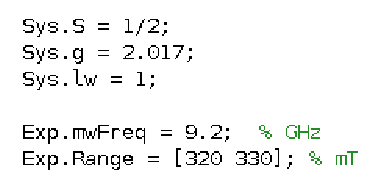
\includegraphics{example_params_fig}}
    \caption[Simple Spin System Definition]{\label{fig:SpinDefinition}
     An example declaration of the basic \textit{EasySpin\index{EasySpin}} struct used in defining the spin system. In this example, `Sys' represents an arbitrary name for the struct, `.S' is the spin parity, `.g' is the g-factor, `.lw' is the ESR\index{Electron Spin Resonance (ESR)}\index{Electron Paramagnetic Resonance (EPR)} line-width, `.mwFreq' is the position of the microwave frequency being probed, and `.Range' is the range of the magnetic field being scanned.}
 \end{figure}

\subsection{Basic Class Structure}

The term `class' is used loosely in this context. Unlike most languages, \textsc{matlab} (and thus \textit{EasySpin\index{EasySpin}}) is based on plain C and thus not really object oriented. However, unlike C, basic class definitions have been added to \textsc{matlab} though they aren't commonly used. \textit{EasySpin\index{EasySpin}} uses a series of `.m' files that represent different abstractions of the overall modeling system that may or may not be implemented in the form of classes. For this thesis, I will use the term `class' to refer to any modular component of the provided \textit{EasySpin\index{EasySpin}} library.

The most notable classes that are supplied with the library are the core plotting functions for ESR\index{Electron Spin Resonance (ESR)}\index{Electron Paramagnetic Resonance (EPR)} spectrums. These include such jocose names as ``garlic" for cw isotropic ESR\index{Electron Spin Resonance (ESR)}\index{Electron Paramagnetic Resonance (EPR)} and ``pepper" for solid state CW ESR\index{Electron Spin Resonance (ESR)}\index{Electron Paramagnetic Resonance (EPR)} (which I will use). Table \ref{fig:EasyFuncs} shows the full list of possible plotting functions supplied in the library. Other functions supplied in Easyspin are mostly related to data import/export, data analysis, and system optimizations.

\begin{table}
\centering
\caption[\textit{EasySpin\index{EasySpin}} functions]{\label{fig:EasyFuncs} List of possible \textit{EasySpin\index{EasySpin}} plotting functions. `\textit{pepper}' is the main function that will be used in this thesis.}
\begin{tabular} {@{\extracolsep{8pt}}rl@{}}
\hline
\hline
Function & Description \\
\hline
garlic & cw EPR\index{Electron Spin Resonance (ESR)}\index{Electron Paramagnetic Resonance (EPR)}, isotropic and fast motion \\
chili & cw EPR\index{Electron Spin Resonance (ESR)}\index{Electron Paramagnetic Resonance (EPR)}, slow motion \\
pepper & cw EPR\index{Electron Spin Resonance (ESR)}\index{Electron Paramagnetic Resonance (EPR)}, solid state \\
salt & ENDOR, solid state \\
saffron & pulse EPR\index{Electron Spin Resonance (ESR)}\index{Electron Paramagnetic Resonance (EPR)}/ENDOR, solid state \\
curry & SQUID magnetometry \\
blochsteady & Bloch equations, steady-state \\
pulse & Shaped pulses \\
esfit & least-squares fitting \\
\hline
\hline
\end{tabular}
\end{table}

In addition to the classes supplied in the \textit{EasySpin\index{EasySpin}} library, I have also built a few of my own for better visualization of spin systems. One such class (which is included in the online repository cited in the introduction) is called ``zeeman.m". This program draws the field splitting of the Zeeman interactions in the spin system over increasing magnetic field. Another class I implemented builds upon this one and is called ``animate.m". This draws the Zeeman diagram and then animates the plot by drawing the resonant magnetic field differences for a given microwave frequency. Again, all of these additional classes are included in an online repository linked to in the introduction of this thesis. 

%\section{Spin Hamiltonians\index{spin Hamiltonian} and Defect-State\index{lattice-defects} Contributions}

\section{Selecting Hamiltonian\index{spin Hamiltonian} Arguments}

In addition to experimentally gathering the ESR\index{Electron Spin Resonance (ESR)}\index{Electron Paramagnetic Resonance (EPR)} data via ODMR\index{Optically Detected Magnetic Resonance (ODMR)}, this thesis is also concerned with emulating the ESR\index{Electron Spin Resonance (ESR)}\index{Electron Paramagnetic Resonance (EPR)} spectrum via EasySpin\index{EasySpin}. However, in order to do this, the Hamiltonian\index{spin Hamiltonian} for each material needs to be understood to the fullest possible extent.

\subsection{ZnO Nanowires}

\begin{table}
\centering
\caption[Spin Parameters]{\label{fig:StehrParams} Summary of the spin-Hamiltonian\index{spin Hamiltonian} parameters for the various defect\index{lattice-defects} centers of ZnO nanowires given by J. E. Stehr et al. The spin-parity and diagonalized g-tensor values are given for each defect\index{lattice-defects} center. For the non-axial centers, $\varphi$ is the angle between the z and c axis.
 \label{stehr_table}}
\begin{tabular}{@{\extracolsep{8pt}}llllllll@{}}
\hline
\hline
& & \multicolumn{2}{c}{Axial} & \multicolumn{3}{c}{Nonaxial} & \\
\cline{3-4}
\cline{5-7}
Center & $S$ & $g_{\bot}$ & $g_{\parallel}$ & $g_{xx}$ & $g_{yy}$ & $g_{zz}$ & $\varphi$ (deg)\\
\hline
$\text{V}_{\text{Zn}}^{-}$ & $1/2$ & $2.0193$ & $2.0024$ & $2.0173$ & $2.0183$ & $2.0028$ & $110.75$ \\
$\text{Z}$ & $1/2$ & $2.006$ & $2.020$ & & & & $20$ \\
$\text{V}_{\text{Zn}}/\text{Zn}_{\text{i}}$ & $1$ & & & $1.9888$ & $1.9893$ & $1.9815$ & $110.75$ \\
$\text{Zn}_{\text{i}}^{+}$ & $1/2$ & $1.9595$ & $1.9605$ & & & & $0$\\
$\text{D}^{*}$ & $1/2$ & $1.9595$ & $1.9605$ & & & & $0$\\
\hline
\hline
\end{tabular}
\end{table}
 
One of the works cited in this thesis investigates the resonant properties of zinc oxide nanowires\ref{NULL}. The author, Stehr, models the ESR\index{Electron Spin Resonance (ESR)}\index{Electron Paramagnetic Resonance (EPR)} spectrum using g-tensor and spin-values given for each defect\index{lattice-defects} center. This data is summarized in table \ref{fig:StehrParams}. Stehr uses the \textit{EasySpin\index{EasySpin}} modeling system to show the predicted ESR\index{Electron Spin Resonance (ESR)}\index{Electron Paramagnetic Resonance (EPR)} spectrum resulting from the $\text{V}_{\text{Zn}}^{-}$, $\text{V}_{\text{Zn}}/\text{Zn}_{\text{i}}$, and $\text{D}^{*}$ defect\index{lattice-defects} center contributions. He models each Hamiltonian\index{spin Hamiltonian} separately using \textit{EasySpin\index{EasySpin}} and then combines the results with \textsc{matlab}. Figure \ref{fig:StehrPlots} shows the plots that he presented to the journal after this process.

\begin{figure}
    \centerline{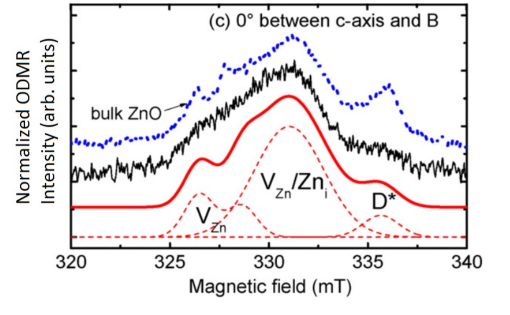
\includegraphics{stehr_fig}}
    \caption[ESR\index{Electron Spin Resonance (ESR)}\index{Electron Paramagnetic Resonance (EPR)} Spectrum Presented by Stehr et al.]{\label{fig:StehrPlots}
     The ESR\index{Electron Spin Resonance (ESR)}\index{Electron Paramagnetic Resonance (EPR)} spectrum presented by Stehr et al. for ZnO Nanowires. The results of computational modeling using \textit{EasySpin\index{EasySpin}} are shown in dashed-red (individual) and solid-red (total). The black line represents actual data from the sample and the blue line is included for comparison to the bulk species.}
 \end{figure}

However, one thing Stehr did not include was the ESR\index{Electron Spin Resonance (ESR)}\index{Electron Paramagnetic Resonance (EPR)} line-width parameters and derivations he used when constructing the spin system via EasySpin\index{EasySpin}. As a verification for the process he used, I have included a reconstruction of the same ESR\index{Electron Spin Resonance (ESR)}\index{Electron Paramagnetic Resonance (EPR)} spectrum that was included in his publication. Through comparison I found that the line-width parameters used by Stehr were $1$, $5$, and $2$ mT for 
$\text{V}_{\text{Zn}}^{-}$, $\text{V}_{\text{Zn}}/\text{Zn}_{\text{i}}$, and $\text{D}^{*}$ respectively. Though it is unknown as to how he arrived at these values, it is likely that he compared the theoretical model to the experimental data until a reasonable fit was achieved. In Figure \ref{fig:StehrRec} I give the recreation of the spectrum and the code used to generate the spin system that Stehr used.


\begin{figure}
    \centerline{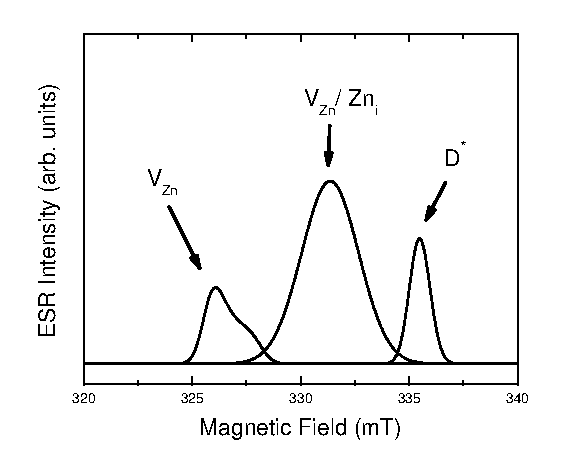
\includegraphics{stehr_rec_fig}}
    \caption[Recreation of ZnO Nanowire ESR\index{Electron Spin Resonance (ESR)}\index{Electron Paramagnetic Resonance (EPR)}]{\label{fig:StehrRec}
     The recreation of the plots given by Stehr et al. for the ZnO nanowire ESR\index{Electron Spin Resonance (ESR)}\index{Electron Paramagnetic Resonance (EPR)} spectrum. All three defect\index{lattice-defects} centers are included as in the original figure. }
 \end{figure}

\subsection{Irradiated 4H-SiC\index{silicon carbide (4H SiC)}}

One of the two primary materials studied in this thesis is silicon carbide\index{silicon carbide (4H SiC)}. In order to compare the theoretical prediction of the ESR\index{Electron Spin Resonance (ESR)}\index{Electron Paramagnetic Resonance (EPR)} spectrum with experimental results we first need to discover what arguments are used in the overall spin Hamiltonian\index{spin Hamiltonian}. Below I have listed the significance and value of each term used in the spin Hamiltonian\index{spin Hamiltonian}. I have also included the pertinent code to represent this system in terms of the aforementioned \textit{EasySpin\index{EasySpin}} struct definition in figure \ref{fig:SiCParams}.

SiC\index{silicon carbide (4H SiC)} is a commonly known to be a spin-3/2 system with two major ESR\index{Electron Spin Resonance (ESR)}\index{Electron Paramagnetic Resonance (EPR)} peaks in its spectrum. The parameter `.S' given for the \textit{EasySpin\index{EasySpin}} system is then just $3/2$. Moreover, as mentioned previously, SiC\index{silicon carbide (4H SiC)} has one major defect\index{lattice-defects} of interest: the silicon divacancy in its lattice structure. The g-factor for this defect\index{lattice-defects} center is given as a rhomboidal two-termed g-factor [$\text{g}_{xx}=\text{g}_{yy}$, $\text{g}_{zz}$] of [$2.003$, $2.0045$]. This is listed as the `.g' parameter in the struct definition.

The linewidths are relatively narrow for specimens related to SiC\index{silicon carbide (4H SiC)}. By comparison to experiment we have found that the full-width-half-maximum value of the line-widths is close to unity. Using \textit{EasySpin\index{EasySpin}} this means that the `.lw' parameter should be set to around $1$

One interesting property of this material is that it exhibits a zero-field splitting which divides the $+3/2$ and $+1/2$ from the $-1/2$ and $-3/2$ states even when there is no external magnetic field. In our definition we have measured this parameter to be about `.D$=450$' MHz at the zero-field marking.

Though it is not readily apparent, SiC\index{silicon carbide (4H SiC)} also exhibits hyperfine splitting in its major ESR\index{Electron Spin Resonance (ESR)}\index{Electron Paramagnetic Resonance (EPR)} peaks. To observe this splitting, two terms can be added to the spin-system: `.A' and '.Nucs'. For SiC\index{silicon carbide (4H SiC)} these two parameters take on the value of `-120` and '29Si' respectively. However, in our example they are insignificant and therefore not included. In Figure \ref{fig:SiCParams} I have commented out these two lines of code to reflect that.

\begin{figure}
    \centerline{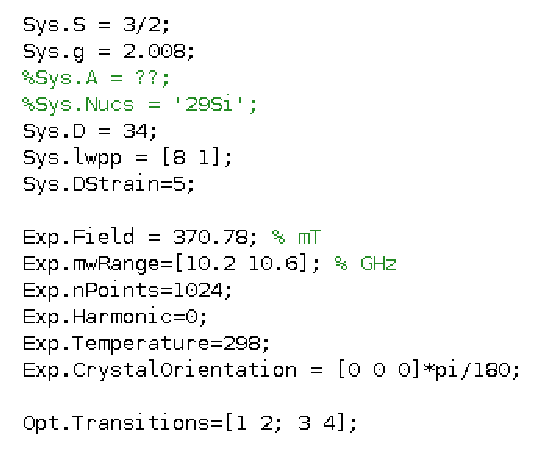
\includegraphics{sic_params_commented_fig}}
    \caption[The \textit{EasySpin\index{EasySpin}} representation of SiC\index{silicon carbide (4H SiC)}]{\label{fig:SiCParams}
     The representation of the known parameters included in the \textit{EasySpin\index{EasySpin}} struct definition for analysis of 4H-SiC\index{silicon carbide (4H SiC)}}
 \end{figure}
 
\subsection{Thin-Film CdTe\index{cadmium telluride (CdTe)}}

[Rough - More] The other material of interest studied in this work is CdTe\index{cadmium telluride (CdTe)}. (Writer's comment: honestly, I may just take anything related to CdTe\index{cadmium telluride (CdTe)} out of my thesis. I don't really have that much information on it to produce good plots.)

[Rough - more] This system exhibits a dominating Cd interstitial defect\index{lattice-defects} (I think. I should look that one up) which contributes a spin-1/2 term to the Hamiltonian\index{spin Hamiltonian}.

[Rough - more] The crystal structure of CdTe\index{cadmium telluride (CdTe)} is (I'll have to look this up) and thus the g-factor included in the Hamiltonian\index{spin Hamiltonian} is (again, i have to look this up).

[Rough - more] I have included the pertinent code to represent this system in terms of the aforementioned \textit{EasySpin\index{EasySpin}} struct definition in figure \ref{fig:CdTeParams}.

\begin{figure}
    \caption[The \textit{EasySpin\index{EasySpin}} representation of CdTe\index{cadmium telluride (CdTe)}]{\label{fig:CdTeParams}
     The representation of the known parameters included in the \textit{EasySpin\index{EasySpin}} struct definition for analysis of thin-film CdTe\index{cadmium telluride (CdTe)}.}
 \end{figure}
 
%\section{Encountered Challenges}










\chapter{Experimental Methods}

The work done for this thesis uses both computational and experimental components in describing ESR. Whereas we described the process of theoretical/computational ESR in the last chapter, we will now describe the experimental-limit of this technique which we call ODMR due to it's optical-coupling of information gathering. This chapter is primarily concerned with detailing the experimental methods implemented in typical ODMR setups. We will also first begin with a qualitative description of the materials we studied (SiC and CdTe).

\section{Sample Preparation}

\subsection{Preparation of Silicon Carbide Samples\index{silicon carbide (4H SiC)}}
\label{sec:SiCSamples}

Three different samples of 4H-SiC\index{silicon carbide (4H SiC)} were provided to us by our collaborator Dr. Sam Carter of the Naval Research lab. Each sample was prepared with a different irradiation fluence to introduce silicon defects into the lattice. The first sample that we tested was irradiated with 2 MeV protons at a fluence of $10^{14} \text{cm}^{-2}$. The second sample was similarly irradiated with 2 MeV protons but at a fluence of $10^{13} \text{cm}^{-2}$. The final sample was an electron-irradiated sample produced with a fluence of $10^{17} \text{cm}^{-2}$. The different strengths of irradiation in each sample is presumed to change the concentration of vacancy defects formed within the sample.

A higher irradiation fluence typically produces a higher concentration of defects. Figure \ref{fig:SiCDepth} shows the distribution of defects in a $10^{12} \text{cm}^{-2}$ sample as a function of spatial depth from the sample's normal face. This data was provided to us by Dr. Sam Carter as part of a ``Stopping and Range of Ions in Matter" (SRIM) study to predict the stopping range for the protons inside this particular species of silicon carbide\index{silicon carbide (4H SiC)} material. From the SRIM calculations, Dr. Carter predicted that the stopping distance of the ions would be at about 44 $\mu$m from the sample's surface. However, further photoluminescence studies showed the concentrations to be closer to about 32 $\mu$m rather than 44 $\mu$m. Finally, each sample was cut such that the c-axis of the lattice was eight degrees from the direction normal to the sample face.

\begin{figure}
    \caption[SiC\index{silicon carbide (4H SiC)} Depth-Dependent Photoluminescence]{\label{fig:SiCDepth}
     Depth-dependent photoluminescence of the $10^{12}$ $\text{cm}^{−2}$ sample at the V2 wavelength. The large peak at 34 $\mu$m indicates the stopping position of the protons. The spatial resolution was 1 $\mu$m.}
 \end{figure}

\subsection{Preparation of Cadmium Telluride Samples}

Like the silicon carbide\index{silicon carbide (4H SiC)}, three different varieties of CdTe\index{cadmium telluride (CdTe)} were prepared for the purpose of our optical study. One was CSS (Caustic Soda Solution) deposited, and two were formed using solution deposition CdTe\index{cadmium telluride (CdTe)} by our collaborator Dr. Mike Scarpulla of the University of Utah. All three samples were produced as a p-type semiconductor and contain vacancy defects\index{lattice-defects} in the crystal-lattice formed through a type of arsenic doping that has been predicted to yield superior results over current techniques commonly used.  

All samples were quite aged and required special surface preparation upon arrival in our lab and did not display adequate photoluminescence intensity due to age-acquired surface recombination velocity. This was reduced using the procedure discussed in \ref{NULL} right before the measurements were taken. refer to \ref{NULL} for the full description of what procedures were used to prep the sample's surface.

\subsection{Photoluminescence data}

As mentioned earlier, ODMR\index{Optically Detected Magnetic Resonance (ODMR)} is a particular type of ESR\index{Electron Spin Resonance (ESR)}\index{Electron Paramagnetic Resonance (EPR)}. The major difference is that ODMR\index{Optically Detected Magnetic Resonance (ODMR)} uses a double-resonance technique to collect ESR\index{Electron Spin Resonance (ESR)}\index{Electron Paramagnetic Resonance (EPR)} data. Because of this, samples had to exhibit adequate resonance in their photoluminescence in order for the absorption of the microwave frequencies to be measured by our detectors. Figures \ref{fig:SiCPL} and \ref{fig:CdTePL} show the photoluminescence spectra of SiC\index{silicon carbide (4H SiC)} and CdTe\index{cadmium telluride (CdTe)} with the pertinent peaks of interest highlighted.

\begin{figure}
    \caption[Photoluminence Spectra of Silicon Carbide]{\label{fig:SiCPL}
      Photoluminence plot showing PL strength vs. wavelength in SiC\index{silicon carbide (4H SiC)}. The peak near 915 nm is the primary peak of interest as it represents the V2 silicon vacancy defect\index{lattice-defects}.}
 \end{figure}
 
\begin{figure}
    \caption[Photoluminence Spectra of Cadmium Telluride]{\label{fig:CdTePL}
     Photoluminence plot showing PL strength vs. wavelength of CdTe\index{cadmium telluride (CdTe)}.}
 \end{figure}

\section{Experiment Background}

The experiments performed in this thesis were performed in tandem with another study involving electron spin coherence in silicon carbide\index{silicon carbide (4H SiC)}. The majority of the equipment used in the spin-studies project was used directly for collecting data for this thesis as well. Because of this, section \ref{sec:Experiment} only summarizes the more important elements and details only those aspects of the experiment that significantly deviate from previous projects. For a more detailed description of the experiment please reference Jacob Embley's undergraduate senior thesis.\ref{NULL}

\section{Experiment Setup}
\label{sec:Experiment}

\begin{figure}
    \centerline{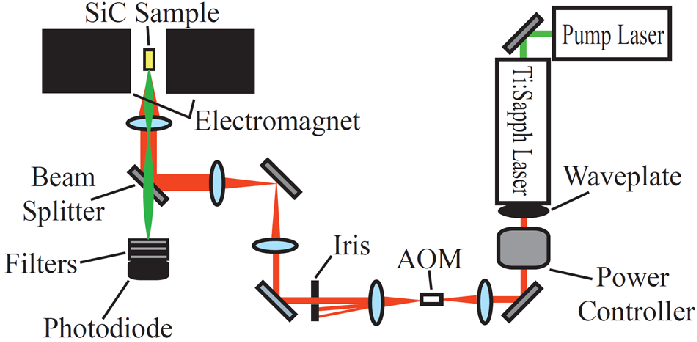
\includegraphics{setup_fig}}
    \caption[Diagram of Experimental Setup for ODMR\index{Optically Detected Magnetic Resonance (ODMR)}]{\label{fig:setup}
     The diagram showing the necessary (labeled) components and arrangement for the ODMR\index{Optically Detected Magnetic Resonance (ODMR)} experiment. A full description of each element is included in section \ref{sec:Experiment}.}
 \end{figure}

The overall setup used in this experiment is shown in Figure \ref{fig:setup}. The basic components necessary to collect ODMR\index{Optically Detected Magnetic Resonance (ODMR)} data are: A laser to stimulate photoluminescence, a constant magnetic field, and an adjustable microwave generator to transition spins between energy levels. Though a cryostat was used, it was not needed and was included as just an artifact for previous experiments that used this same setup. For our purposes the cryostat kept the sample at a constant room-temperature for consistency in the experiment. These components are described in detail in the next section.

\subsection{Temperature Controller and Static Magnetic Field}

All samples studied were held at constant temperature and magnetic field. A nonmagnetic \textit{CryoIndustries} cryostat was used to maintain constant temperature on the sample throughout the duration of the experiments. A turbopump was used in conjunction with the cryostat to keep the pressure around $10^{-5}$ mbar. A PID \textit{CryoCon} controller was used as the heating element in the chamber. When used in combination with the cryostat, any temperature between 8 K and 300 K could be achieved. Many different temperatures of ODMR\index{Optically Detected Magnetic Resonance (ODMR)} were recorded for the samples between these two temperatures.

Most ESR\index{Electron Spin Resonance (ESR)}\index{Electron Paramagnetic Resonance (EPR)}\index{Electron Spin Resonance (ESR)}\index{Electron Paramagnetic Resonance (EPR)}-type experiments hold microwave frequency constant and sweep magnetic field strength, but for our purposes it was easier to do this in the reverse manner. As our data shows, the results can be interpreted the same way for either method. An external static magnetic field of 0.37 T was applied constantly throughout the experiment. A large iron-core electromagnet was powered using a Magna-Power Electronics TS Series IV power supply. A Lakeshore DSP 750 gaussmeter was used as a PID controller to make fine adjustments to the magnetic field so that it stayed constant at 0.37 T.

\subsection{Laser and Optics}

In order for photoluminescence to be measured off the sample, a laser must first stimulate the sample. The laser used for this experiment was a 3900 S Ti:Sapph laser tuned to 870 nm and pumped by a 532 nm solid diode laser. The Ti:Sapph was focused to around 50 micrometers and controlled by a Brockton Electro-Optics Corp BEOC laser power controller. The laser was chopped with a NEOS Technology 15210 acousto-optic modulator (AOM) and paired with a Stanford Research System lock-in amplifier recording filtered light from a photodiode.

\subsection{Microwave Generation and Amplification}

Microwaves induce transitions between the Zeeman energy levels and are the fundamental variable modulated to retrieve ODMR\index{Optically Detected Magnetic Resonance (ODMR)} data. The microwaves used for this experiment were produced using an Agilent Technologies E8257D microwave generator set at 10.4855 GHz at 0 dBm. A 20T4G18 traveling wave tube microwave amplifier increased the power of the microwaves up to about 40 dBM. The microwaves were then fed to a coupling loop placed next to the sample within the cryostat.

\subsection{Software Controller Interfaces and Data Recording}

All experiments were conducted using a LabVIEW suite of programs designed to succinctly gather and record ODMR\index{Optically Detected Magnetic Resonance (ODMR)} data. For our experiment, the LabVIEW suite controlled the microwave and laser modulating so that both could be referenced with a lock-in amplifier as necessary. The microwave generator and lock-in amplifier were interfaced using a GPIB addressing bus implemented as a separate class instantiation in the main LabVIEW program. The instrument classes were all designed to run in parallel to the main scanning software for better experiment control. The generic scanner object was built to handle an abstracted object implementing a ``scannable" interface and another object implementing a ``readable" interface. The scanner was built robustly enough to handle any combination of instrumentation that inherits from these two interfaces. It gives directives to the ``scannable" object while also recording data from the ``readable" object at the same time. A beta version of the program is linked-to in the introduction of this thesis and represents the ongoing work of myself, Ryan Peterson, Kyle Miller, Phil White, John Colton, and others.

In addition to the main LabVIEW suite of programs used, an additional PID-controller VI was built to run on its own thread. This was used to handle the magnetic field strength incident on our sample and make minor adjustments to the power-supply for the magnet according to measurements read off of the gaussmeter inserted into the field.

The overall program accepts as input a range of microwave frequencies and then records the absorption from the sample representing the ODMR\index{Optically Detected Magnetic Resonance (ODMR)}. After this data was recorded, a graphing software known as \textit{Origin} was used to produce plots from the raw data. No other data analysis was needed apart from the straight reproduction of the raw data into readable plots. The concluding chapter shows these results.










\chapter{Results}

\section{Computational Predictions}

\begin{figure}
    \caption[ODMR\index{Optically Detected Magnetic Resonance (ODMR)} computational model for SiC\index{silicon carbide (4H SiC)}]{\label{fig:SiCModel}
     This is the figure description.}
 \end{figure}

\begin{figure}
    \caption[ODMR\index{Optically Detected Magnetic Resonance (ODMR)} computational model for CdTe\index{cadmium telluride (CdTe)}]{\label{fig:CdTeModel}
     This is the figure description.}
 \end{figure}

\section{Experimental Results}

\begin{figure}
    \caption[Experimental ODMR\index{Optically Detected Magnetic Resonance (ODMR)} for SiC\index{silicon carbide (4H SiC)}]{\label{fig:SiCResults}
     This is the figure description.}
 \end{figure}

\begin{figure}
    \caption[Experimental ODMR\index{Optically Detected Magnetic Resonance (ODMR)} for CdTe\index{cadmium telluride (CdTe)}]{\label{fig:CdTeResults}
     This is the figure description.}
 \end{figure}


\section{Data Analysis}

\section{Conclusion}

\begin{appendices}











\chapter{Electron Spin Studies of Electron Irradiated SiC\index{silicon carbide (4H SiC)}}
\label{chpt:AppendA}

\begin{figure}
    \caption[Electron-irradiated SiC\index{silicon carbide (4H SiC)} lifetime  summary]{\label{fig:e17results}
     This is the figure description.}
 \end{figure}

\begin{figure}
    \caption[ODMR\index{Optically Detected Magnetic Resonance (ODMR)}/Photoluminescence vs temperature]{\label{fig:ODMRPL}
     This is the figure description.}
 \end{figure}











\chapter{Optical Studies of Cadmium Telluride}
\label{chpt:AppendB}









\chapter{Electron Spin Coherence of Silicon Vacancies in Proton-Irradiated 4H-SiC\index{silicon carbide (4H SiC)}}
\label{chpt:AppendC}

\end{appendices}

word
\cite{RefWorks:doc:58929816e4b0499fa95c51a6}
\cite{RefWorks:doc:58929629e4b0d4c09201f6b8}
\cite{RefWorks:doc:589299f4e4b0d4c09201f915}
\cite{RefWorks:doc:58929128e4b0228a292928a7}
\cite{RefWorks:doc:589299fbe4b0dec22aee3bd8}
\cite{RefWorks:doc:5892912ae4b0dec22aee3993}
\cite{RefWorks:doc:58929128e4b0499fa95c5064}
\cite{RefWorks:doc:5892989ee4b0499fa95c51c8}
\cite{RefWorks:doc:589293f5e4b0dec22aee39de}
\cite{RefWorks:doc:589295fce4b0d4c09201f6b4}
\cite{RefWorks:doc:58929a02e4b0d4c09201f91b}
\cite{RefWorks:doc:589295bde4b0d4c09201f692}
\cite{RefWorks:doc:58929264e4b0d4c09201f63b}
\cite{RefWorks:doc:58929129e4b0d4c09201f61e}
\cite{RefWorks:doc:58929602e4b0d4c09201f6b6}
\cite{RefWorks:doc:589296c6e4b0d4c09201f6f5}
\cite{RefWorks:doc:58929746e4b0dec22aee3a9a}
\cite{RefWorks:doc:589297a9e4b0d4c09201f736}
\cite{RefWorks:doc:58929800e4b0499fa95c51a1}
\cite{RefWorks:doc:589299f0e4b0dec22aee3bd6}
\cite{RefWorks:doc:58929786e4b0228a292929b8}
\cite{RefWorks:doc:58929612e4b0499fa95c50fa}
\cite{RefWorks:doc:5892964ee4b0499fa95c5108}
\cite{RefWorks:doc:58929c15e4b0228a29292c58}
\cite{RefWorks:doc:5892912ae4b0228a292928aa}

\begin{figure}
    \centerline{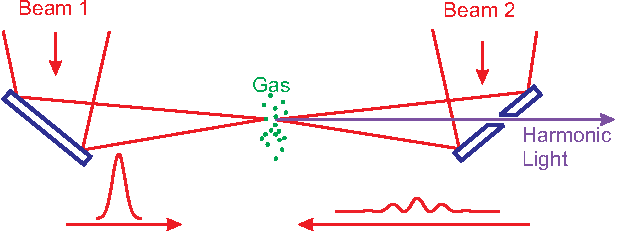
\includegraphics{Graphic1}}
    \caption[Setup for using counter-propagating light]{\label{fig:MirrorDiagram}
     A mirror with a hole is used to extract high-order harmonics generated in
     counter-propagating laser beams.}
\end{figure}

\begin{figure}
    \caption[SiC\index{silicon carbide (4H SiC)} energy levels and zero-field splitting]{\label{fig:SiCZeeman}
     This is the figure description.}
 \end{figure}





% Make the bibliography.
% Enter your references in the BibTex file "references.bib"
\bibliography{references}

% Make the index
\printindex

\end{document}
